% This work is made available under the terms of the
% Creative Commons Attribution-ShareAlike 4.0 license,
% http://creativecommons.org/licenses/by-sa/4.0/.
%
% Version: $Revision$

\documentclass[a4paper]{book}

\usepackage{wrapfig}
\usepackage{graphicx}
\usepackage{hyperref}
\usepackage{multirow}
\usepackage{scalefnt}
\usepackage{tikz}

% watermark -- for draft stage
\usepackage[firstpage]{draftwatermark}
\SetWatermarkLightness{0.9}
\SetWatermarkScale{5}

% Copyright (c) 2009 by the University of Waikato, Hamilton, NZ. 
% This work is made available under the terms of the 
% Creative Commons Attribution-ShareAlike 4.0 license,
% http://creativecommons.org/licenses/by-sa/4.0/.
%
% Version: $Revision: 5479 $

\newenvironment{tight_itemize}{
\begin{itemize}
  \setlength{\itemsep}{1pt}
  \setlength{\parskip}{0pt}
  \setlength{\parsep}{0pt}}{\end{itemize}
}

\newenvironment{tight_enumerate}{
\begin{enumerate}
  \setlength{\itemsep}{1pt}
  \setlength{\parskip}{0pt}
  \setlength{\parsep}{0pt}}{\end{enumerate}
}

% if you just need a simple heading
% Usage:
%   \heading{the text of the heading}
\newcommand{\heading}[1]{
  \vspace{0.3cm} \noindent \textbf{#1} \newline
}

\newcommand{\icon}[1]{\tikz[baseline=-3pt]\node[inner sep=0pt,outer sep=0pt]{\includegraphics[height=1.1em]{#1}};}


\title{
  \textbf{ADAMS} \\
  {\Large \textbf{A}dvanced \textbf{D}ata mining \textbf{A}nd \textbf{M}achine
  learning \textbf{S}ystem} \\
  {\Large Module: adams-twitter} \\
  \vspace{1cm}
  
\includegraphics[width=2cm]{images/twitter-bird-blue-on-white.png} \\
}
\author{
  Peter Reutemann
}

\setcounter{secnumdepth}{3}
\setcounter{tocdepth}{3}

\begin{document}

\begin{titlepage}
\maketitle

\thispagestyle{empty}
\center
\begin{table}[b]
	\begin{tabular}{c l l}
		\parbox[c][2cm]{2cm}{\copyright 2012-2015} &
		\parbox[c][2cm]{5cm}{
\includegraphics[width=5cm]{images/coat_of_arms.pdf}} \\
	\end{tabular}
	
\includegraphics[width=12cm]{images/cc.png} \\
\end{table}

\end{titlepage}

\tableofcontents
\listoffigures
%\listoftables

%%%%%%%%%%%%%%%%%%%%%%%%%%%%%%%%%%%
\chapter{Introduction}
ADAMS is a great environment for processing data streams. Using the excellent
Java library \textit{twitter4j} \cite{twitter4j}, you can tap into Twitter's 
stream of tweets or query for tweets that meet certain criteria.

\begin{figure}[htb]
  \centering
  
\includegraphics[width=3.0cm]{images/twitter-bird-blue-on-white.png}
\end{figure}

%%%%%%%%%%%%%%%%%%%%%%%%%%%%%%%%%%%
\chapter{Flow}
The flow comes with a range of actors for accessing the Twitter API.

\noindent The following standalone actors are available:
\begin{tight_itemize}
	\item \textit{TwitterConnection} - here you set up your parameters, like 
	consumer key/secret. It uses the globally defined preferences as default
	parameters (see chapter \ref{preferences}).
\end{tight_itemize}

\noindent The following sources are available:
\begin{tight_itemize}
	\item \textit{TwitterListener} - listens to the \textit{sample} stream
	of tweets.\footnote{adams-twitter\_listener1.flow, adams-twitter\_listener2.flow}
	\item \textit{TwitterQuery} - retrieves tweets that match your 
	query.\footnote{adams-twitter\_query1.flow, adams-twitter\_query2.flow, adams-twitter\_query3.flow}
\end{tight_itemize}

\noindent The following transformers are available:
\begin{tight_itemize}
	\item \textit{TwitterConverter} - turns the tweets into a different format
	using the specified converter (e.g., text or spreadsheets).
	\item \textit{TwitterFilter} - allows you to filter the stream of tweets
	coming through using a filter expression. Useful when generating several
	datasets with different subsets (in sub-branches) from the same stream 
	of tweets.\footnote{adams-twitter\_query4.flow}
\end{tight_itemize}

\noindent The following sinks are available:
\begin{tight_itemize}
	\item \textit{Tweet} - updates your status with the incoming string.
\end{tight_itemize}

\noindent The following boolean conditions are available (can be used in 
\textit{IfThenElse} or \textit{Switch} control actors):
\begin{tight_itemize}
	\item \textit{TwitterFilterExpression} - allows to perform checks on the 
	status object passing through.\footnote{adams-twitter\_query4.flow, adams-twitter\_query5.flow}
\end{tight_itemize}

For more information on the format of search queries used by the
\textit{TwitterQuery} source, see the following URL: \\
\url{https://dev.twitter.com/rest/public/search}{}

%%%%%%%%%%%%%%%%%%%%%%%%%%%%%%%%%%%
\chapter{Preferences}
\label{preferences}
The \textit{TwitterConnection} standalone actor uses the globally defined
twitter setup for its default settings. If you don't want to hand out your
keys and secrets, you can simply configure your keys/secrets in the global
settings and just use the default \textit{TwitterConnection} configuration.
Figure \ref{twitter_preferences} shows the preferences tab for Twitter.
\begin{figure}[htb]
  \centering
  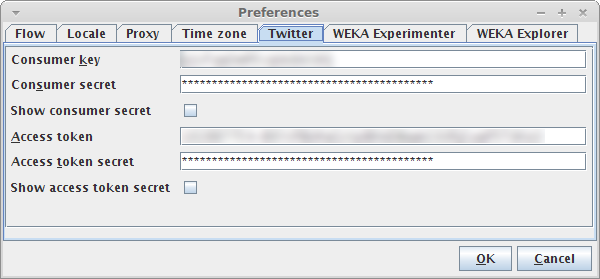
\includegraphics[width=8.0cm]{images/twitter_preferences.png}
  \caption{Twitter preferences}
  \label{twitter_preferences}
\end{figure}

%%%%%%%%%%%%%%%%%%%%%%%%%%%%%%%%%%%
% Copyright (c) 2009-2012 by the University of Waikato, Hamilton, NZ. 
% This work is made available under the terms of the 
% Creative Commons Attribution-ShareAlike 4.0 license,
% http://creativecommons.org/licenses/by-sa/4.0/.
%
% Version: $Revision$

\begin{thebibliography}{999}
	% to make the bibliography appear in the TOC
	\addcontentsline{toc}{chapter}{Bibliography}

    % references
	\bibitem{adams}
		\textit{ADAMS} -- Advanced Data mining and Machine learning System \\
		\url{https://adams.cms.waikato.ac.nz/}{}
		
	\bibitem{heatmap}
		\textit{Heat map} -- WikiPedia article \\
		\url{http://en.wikipedia.org/wiki/Heat_map}{}

\end{thebibliography}


\end{document}
